\documentclass{article}
\usepackage{fontspec}
\usepackage{jim}
\usepackage{amsmath}
\usepackage[french]{babel}
\usepackage{listings}
\usepackage{diagbox}
\usepackage{caption}
\usepackage{booktabs}
\usepackage{microtype}
\usepackage{graphicx}
\usepackage{hyperref}
\usepackage{tikz}
\usepackage{xspace}
\usepackage{array}
\usepackage{subcaption}
\usepackage[backend=biber]{biblatex}
\addbibresource{biblio.bib}

\setmainfont{Tribun ADF Std}

\newcolumntype{C}[1]{>{\centering\arraybackslash}m{#1}}   %% centered
\newcolumntype{R}[1]{>{\raggedright\arraybackslash}m{#1}}  %% right aligned
\newcolumntype{L}[1]{>{\raggedleft\arraybackslash}m{#1}}  %% right aligned

\newcommand\timenode{nœud temporel\xspace}
\newcommand\trigger{point d'interaction\xspace}
\newcommand\triggers{points d'interaction\xspace}
\newcommand\vocab[1]{\textbf{#1}}
\DeclareCaptionType{scenario}[Scénario]
% Title.
% ------
\title{Écriture et exécution répartie de scénarios interactifs}

\threeauthors
  {Auteur 1} {Organisme \\ Adresse électronique}
  {Auteur 2} {Organisme \\ Adresse électronique}
  {Auteur 3} {Organisme \\ Adresse électronique}

\begin{document}
\maketitle
\begin{abstract}
    La pratique musicale est souvent une opportunité pour interagir et échanger, 
    avant tout avec d'autres musiciens, et plus récemment avec des algorithmes ou logiciels 
    disposant d'un certain degré d'autonomie et de liberté.
    
    La notation musicale occidentale résout le problème du partage et de la séparation d'information entre musiciens 
    en divisant une partition en portées; la plupart des logiciels musicaux vont interpréter ces portées sur une seule machine, en gardant la possibilité de pistes avec des réglages indépendants. 
    
    Ce travail consiste en une généralisation de cette notion de partage aux scénarios interactifs, en permettant une exécution synchrone ou asynchrone de plusieurs parties d'un scénario sur plusieurs machines.
    Une implémentation est offerte dans le logiciel i-score, avec pour objectif de mettre en valeur 
    les nouvelles possibilités d'écriture qu'offre une exécution répartie à un compositeur.
\end{abstract}
\section{Problématique}
On cherche à définir une sémantique permettant de décrire l'exécution d'une partition interactive sur plusieurs machines, en prenant en compte les exécutions parallèles, c'est-à-dire que deux machines jouent la même chose, de manière synchronisée ou non, ainsi que les exécutions série : une machine joue puis une autre machine joue la suite.

On parle ici de «jeu» à un niveau abstrait~: on s'intéresse au contrôle de tous types de paramètres et non pas uniquement les paramètres musicaux.

On présentera d'abord plusieurs applications et besoins rencontrées par des artistes et auteurs, qui ont motivé ce travail.
Puis, les possibilités de répartition étudiées seront présentées dans le détail, en analysant l'impact que peuvent avoir les problèmes connus dans le domaine de l'informatique répartie, sur l'écriture de telles partitions. 
Pour conclure, les performances du système développé seront présentées.

%TODO notation graphique pour groupes, synchrone, asynchrone, etc... ?
\section{Études de cas}

\subsection{Projet Quarrè}
Quarrè (fig.~\ref{img.quarre}) est une installation en son spatialisé réalisée par Pierre Cochard au SCRIME, qui utilise Max/MSP, i-score, et une application mobile développée pour l'occasion. 
Elle implique plusieurs participants possédant chacun un téléphone.

Une trame principale d'environ trente minutes se déroule.
Durant cette trame, à différents moments, des participants vont pouvoir interagir via l'application mobile, qui les avertis par un compte à rebours. 
Ils disposent ensuite d'une durée déterminée pour agir : changer un paramètre d'un effet, déclencher des sons, spatialiser un objet sonore\dots 
Les actions possibles varient en fonction du nombre de participants, pouvant aller de un à cinq.

%- Cas des applis de téléphone : un objet qui s'exécute sur plusieurs machines en parallèle (dont on veut aggréger les résultats)

\begin{figure}[h]
    \centering
    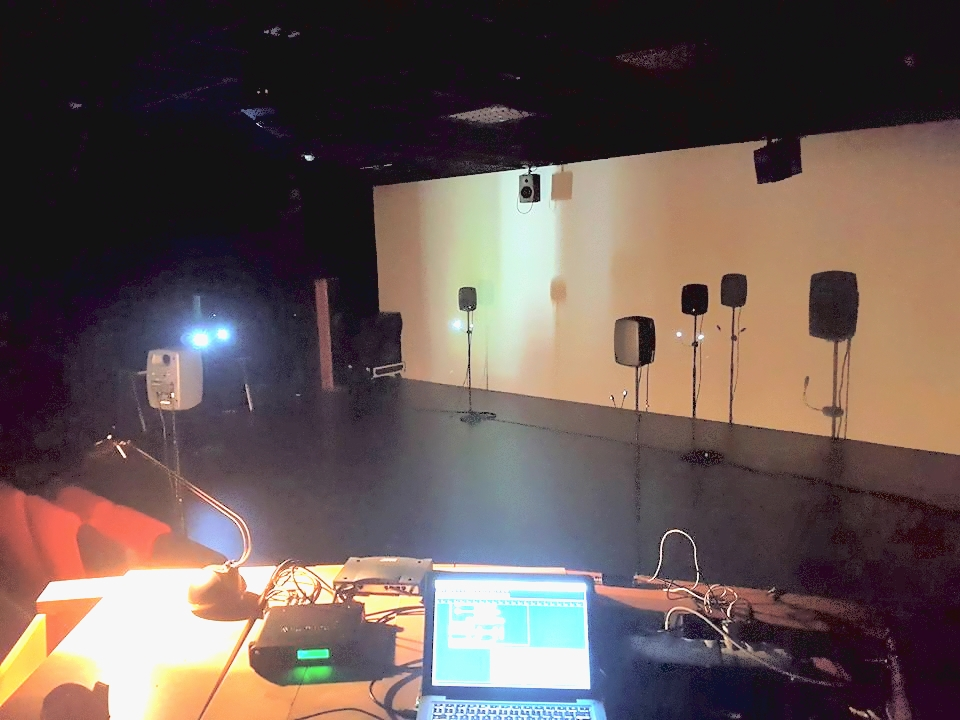
\includegraphics[scale=0.2]{images/quarre.jpg}
    \caption{Quarrè sans participants. Pierre Cochard, 2016.}
    \label{img.quarre}
\end{figure}

\subsection{Support des périphériques embarqués}
Actuellement, une des manières principales d'utiliser le logiciel i-score est de lui faire faire du contrôle par réseau. 

Néanmoins, sur des périphériques embarqués, cela a un coût : 
\begin{itemize}
    \item Encombrement de la bande passante : certains périphériques ne sont pas en Gigabit Ethernet; envoyer des quantités importantes de messages OSC sur des intervalles de quelques millisecondes va entraîner des pertes de paquets, des retards et l'augmentation du temps de latence.
    \item Gigue\footnote{De l'anglais \textit{jitter}} sur les messages envoyés qui peut entraîner des effets indésirables comme des tremblements si par exemple on fait se déplacer des objets graphiques par réseau.
    \item Consommation de ressources pour le décodage des messages réseaux.
\end{itemize}

De plus, actuellement, il est nécessaire de copier les fichiers de sauvegarde sur le périphérique à chaque modification que l'on veut tester, ce qui est peu ergonomique. 
On essaye donc par la même occasion d'offrir un système qui permette de partager automatiquement un scénario i-score entre deux machines.

\subsection{Lecture de médias synchronisée}
On désire offrir des possibilités de lecture vidéo permettant à 
des clips audio ou vidéo de démarrer au même instant sur plusieurs machines, 
puis de rester synchronisés durant la lecture.

\subsection{Redondance}
Le matériel n'étant pas infaillible, la question de la résilience se pose~: comment mitiger une panne de l'ordinateur principal pendant une représentation artistique ?

Une des possibilités est d'offrir un système de redondance : si une machine tombe en panne, une autre prend le relais le plus vite possible.
La machine prenant le relai doit donc avoir été préalablement synchronisée avec la machine étant tombé en panne, pour garantir le moins de perturbations possibles.
 
%- Donner la possibilité de faire un dialogue (boucle avec un coup un \trigger qui vient de A, un coup un \trigger qui vient de B, etc)
%- Approche alternative avec application mobile.

\subsection{État de l'art}
\subsubsection{Rappel du modèle d'i-score}
\cite{celerier2015ossia}
Vocabulaire. Prendre article SMC.

Mettre accent sur hiérarchie
%\subsubsection{Répartition à l'édition}
\subsubsection{Répartition à l'exécution}
%\subsubsection{Lien entre la répartition à l'édition et la répartition à l'exécution}


\subsubsection{Horloges}
Problème de l'horloge : 
\begin{itemize}
\item Si on utilise l'horloge système, pas de garantie qu'elle soit bien synchronisée. 
Et NTP pas dispo partout (on n'a pas forcément les droits sur un téléphone pour changer l'heure).
Horloge i-score se resynchronise déjà en cas de délai sur une machine.
\item Si on utilise une horloge interne, problème de la synchronisation avec l'horloge système (pour le tick)
\end{itemize}

\url{http://queue.acm.org/detail.cfm?id=2745385}
\url{http://radar.oreilly.com/2012/10/google-spanner-relational-database.html}
\url{http://www.ntp.org/ntpfaq/NTP-s-sw-clocks-quality.htm}

Faire la relation entre notre système et le problème CAP : \url{https://en.wikipedia.org/wiki/PACELC_theorem}

Horloges logiques : équivalent à envoyer une timestamp à chaque tick (on arrive donc à un méchanisme de vector clock approximatif). 

Synchro d'horloges de deux clionts dont une qui ralenti, si elles exécutent le même 
scénario ? Il faut les recaler régulièrement. 

Possibilité : externe (NTP, etc) ou interne : \url{https://github.com/ethanlim/NetworkTimeProtocol}

Recaler dès qu'on accumule du retard ?



On peut introduire un recalage sur la master clock entre chaque tick.

Ce qu'on fait : ping régulier vers chaque client (toutes les 100 millisecondes)

Quand quelque chose doit se synchroniser, on dit à chaque client à quel instant il est supposé arriver par rapport à son horloge système.

Quand un client reçoit un ordre pour un timenode à t, il l'applique dès que t <= local(t) (modulo un tick?)



Possibilité : synchronisation via démon externe (PTP, NTP...), mais pas toujours possible (on ne peut pas supposer que l'utilisateur a les droits pour changer l'horloge sur sa machine).

Synchronous ethernet

Ableton Link : synchro sur les ticks musicaux 

Avoir une horloge propre à i-score ? Mais du coup maintenant il faut la synchroniser à l'horloge système. 

\subsubsection{Problématique de la sécurité}
On veut : résistance aux "normal" failures, pas Byzantine failures.

\subsubsection{Synchronisation de médias}
- pas pour l'instant... doivent être au même endroit sur la même machine.
Ableton Link ? Netjack ?

\section{Approche}
Cette section détaille les choix de haut niveau réalisés.

On souhaite modifier le moins possible le modèle pour les utilisateurs du logiciel, 
en rajoutant les notions nécessaires et suffisantes pour offrir la finesse de répartition désirée.

La section~\ref{sec.description} présente de manière détaillée les possibilités 
de répartition que l'on offre, en prenant example sur des cas simples.

La section~\ref{sec.semantique} définit ces possibilités en utilisant les objets du modèle d'i-score. 
On notera que cette méthode serait prohibitoire à réaliser manuellement~: c'est un modèle pour réaliser l'implémentation, qui se fait automatiquement à partir de la spécification que donne le compositeur via les outils présentés en section~\ref{sec.description}. 
On prendra donc garde à ne pas confondre la forme de répartition qui existe déjà de fait dans le logiciel, l'objectif premier d'i-score étant de communiquer avec d'autres logiciels, de la répartition entre instances d'i-score partageant un même document.

Enfin, la section~\ref{sec.evaluation} présente une évaluation des performances dans le cadre 
d'une implémentation pratique.

-------------------------------------------
Première approche basées sur réseau de Pe-tri.

Puis migration du modèle d'i-score maintenant autonome.


- Problème des devices. Note : si on se permet d'envoyer des messages OSC quelconques (i.e. pas dans l'arbre), ça peut simplifier des choses. Aussi, permettre devices qui sont juste en mode envoi ? Il faut un autre proto que OSC ou Minuit...

Aussi, refactoriser pour utiliser tout i-score en librairie

Différentes possibilités de répartition sont disponibles selon les types de processus.

Détailler les implications des choix par rapport au théorême CAP et PACELT.

\subsection{Nouvelles notions}
Nous nous trouvons en présence de plusieurs machines qui communiquent et partagent un document.
L'ensemble constitué par les instances d'i-score et le document qu'elles partagent est appelé \vocab{session}.

On désigne par \vocab{client} une instance d'i-score connectée à une session.

On désire s'affranchir des notions propres aux machines physiques et des problématiques de réseau (addresse IP, etc) lors de l'écriture 
d'un scénario réparti. 

Pour ce faire, on introduit la notion de \vocab{groupe}. 
Un groupe est un ensemble de clients.

Les compositeurs ne manipulent jamais directement la notion de client, uniquement celle d'un groupe qui peut contenir zéro, un, ou plusieurs clients.

De manière générale, quand plusieurs clients font partie d'un même groupe, cela signifie qu'ils vont réaliser les mêmes tâches, de manière synchrone ou asynchrone.

L'intérêt d'un groupe est la tolérance aux pannes, déconnections, reconnections, et changements d'installation. 
Par exemple, si une machine tombe en panne, on peut la remplacer par une autre simplement en l'assignant au même groupe que la machine en panne 
sans avoir besoin de mettre à jour le scénario.


\begin{figure}[h]
	\centering
	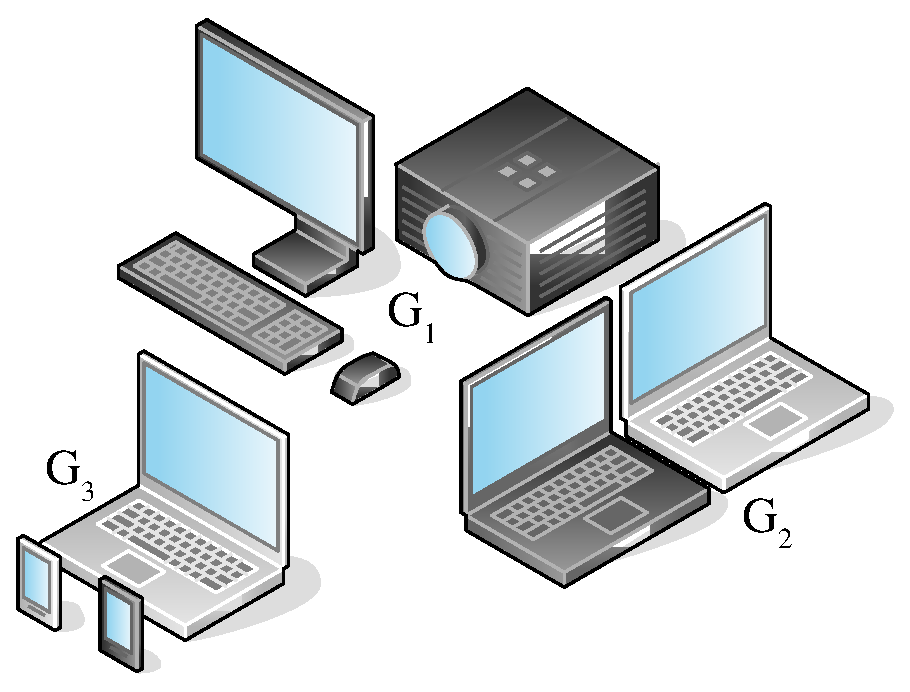
\includegraphics[scale=0.2]{images/groupes.eps}
	\caption{Plusieurs groupes $A,B,C$ avec plusieurs clients dans chaque groupe}
	\label{img.groupes}
\end{figure}


\subsection{Topologie}
Maître-esclave pour l'édition.

Pour des raisons de simplicité, la première mise en œuvre se fait via une toplogie réseau en étoile : un maître gère 
le déroulement général de l'exécution. 
Les différents clients communiquent au travers de ce maître, avec les avantages et inconvénients que cela implique : 
\begin{itemize}
	\item Facilité d'analyse lors du développement : on peut enregistrer tous les messages échangés avec leurs estampilles.
	\item Intolérance aux pannes : si le maître faillit, aucune récupération n'est possible.
\end{itemize}

On détaille dans les sections suivantes les cas ou des topologies différentes peuvent montrer un intérêt.

Pour l'exécution : dans certains cas deux clients peuvent échanger directement.
Il faut décrire ces cas.

Si groupes avec plusieurs clients : "group leader" ? responsable de la communication ? avoir un "plus court chemin" permanent ?

\subsection{Modèle}
i-score se base sur une approche orientée document.

On choisit de répartir nos objets autour d'un même document partagé par toutes les instances du réseau, 
à la manière des logiciels d'édition tels que Google Docs. %CITE

Cela ne pose pas de problème de mémoire, même sur de l'embarqué tel que Raspberry Pi : l'empreinte mémoire d'un scénario est minime en comparaison de l'occupation des bibliothèques utilisées (quelques dizaines de kilo-octets contre environ 50 méga-octets).

On utilise le protocole TCP pour tous les messages relatifs à la répartition, notamment pour ses garanties d'ordonnancement.
\subsection{Répartition de l'édition}
- Partage de file undo - redo. Transformations opérationnelles. %CITE

- Autres approches : partage du modèle lui-même.

- Pour l'édition temps-réel, on doit permettre d'appliquer des "filtres" (par exemple qui vont rajouter une sur-expression, etc)

\section{Description de l'exécution}\label{sec.description}
On sépare les objets offrant une structure temporelle, des objets possédant des données et commandes envoyées à d'autres logiciels (par exemple, une automation).

Des groupes et des méthodes de synchronisation sont assignées à ces objets par le compositeur; en pratique, ces informations sont enregistrées comme une liste de méta-données associées aux objets.
Il est possible d'assigner plusieurs groupes à un objet; cela se comporte comme un groupe constitué de la somme des clients de chaque groupe était assigné.

% *** est-ce que ce n'est pas plus intéressant d'essayer de spécifier le cas ou on a plusieurs groupes sur plusieurs objets ? 
\subsection{Processus de contenu}
On entend par processus de contenu, tous les processus produisant des données, sans se soucier de la structuration temporelle. En voici une liste non exhaustive : automation, mapping, code javascript, piano roll MIDI, audio\dots

Le processus s'exécute tel quel pour tous les clients auquel il est assigné, 
et ne s'exécute pas pour les autres.

Ici les processus de contenu sont représentés par une boite barrée en diagonale, qui représente le cas courant d'une automation montante.
% TODO pour devices, faire en sorte que les clients ne se connectent que à ceux qui sont en local ? Ou même mode "non connecté" (mais impossible de recevoir comme ça). Ou bien avoir une "map" d'addresse ip / port pour chaque paire client <-> device.

\subsubsection{Comportements de groupes}
-> pourquoi ne pas avoir la même chose au niveau des mappings (et pour tout ce qui n'est pas fixé de manière générale ?)
Deux manières : offrir un processus de mapping spécialisé qui permet de définir les relations qu'on veut dans un groupe ("first", "all", "mean", "sum", etc...)

Ou bien faire cette transformation à plus bas niveau (pour les devices) : les sorties sont constantes mais on peut appliquer des transformations aux entrées.
Par exemple, si on possède un device spécial "network" avec l'arbre local de chaque "groupe", qui offre une couche d'abstraction au-dessus des méchanismes de consensus, on peut avoir des possibilités plus riches, telles que : l'expression $e_2$ est vraie si l'expression $e_1$ était vraie pour le groupe $B$ et fausse pour le groupe $A$.

Pour permettre plus de possibilités, on introduit la possibilité de réaliser des expressions qui réalisent un pattern-matching : 
\lstinline|network:/*/trigger == true|.

\subsection{Processus Scénario}
Le scénario est le processus central d'i-score : il met en relation les différents éléments temporels.

Plusieurs manières de répartir l'exécution d'un scénario, offrant différentes possibilités d'écriture, sont détaillées ci-dessous. On sépare le cas général permettant l'interactivité dans un scénario (le scénario continue après qu'un évènement externe $e$ se soit déclenché, visible par exemple en scénario~\ref{scenar.general}) du cas plus simple ou les dates sont fixées, visible en scénario~\ref{scenar.non-interactif}.

On travaillera dans les examples suivants avec trois groupes $A,B,C$ disposant chacun d'un nombre inconnu de clients. 
On pourra supposer que les contraintes temporelles portent chacune des processus de contenus, qui ne sont pas représentés ici afin de garder les figures simples.

\subsubsection{Modes de synchronisation}
On identifie trois niveaux de synchronisation, qui peuvent chacuns avoir leur utilité dans un cas différent : 
\begin{itemize}
    \item Asynchrone : lorsqu'une information interactive est disponible dans le système (par exemple «une expression se vérifie»), elle est propagée le plus vite possible aux autres noeuds qui doivent appliquer le résultat de cette information. Ce mode ne respecte pas nécessairement la sémantique avant-après de i-score mais permet de réduire la latence.
    \item Synchrone : lorsqu'une information est disponible dans le système, elle est propagée de manière à ce que la date absolue de réalisation soit  la même (pour un observateur externe) pour tous les clients. 
    Ce mode respecte la sémantique de i-score~: les éléments s'exécutent dans le même ordre que si le scénario n'était pas réparti, au prix d'une latence augmentée.    
    Il convient de rappeler qu'il est physiquement impossible d'exécuter les objets avec la même précision temporelle que s'ils étaient exécutés dans un même tic d'horloge sur le même client: l'objectif est de minimiser les décalages temporels.
    \item Précalculé : ce mode est surtout utile dans le cas non-interactif : dès qu'une date peut être fixée, elle l'est, et les clients n'attendent pas de message annonçant la fin. 
    Plus la synchronisation des horloges sera fine entre les clients et plus ce mode se rapprochera de l'exécution dans le cas non réparti.
\end{itemize}

Les différents modes de synchronisation vont impacter : 
\begin{itemize}
    \item L'exécution des \triggers.
    \item La vérification de la validité des conditions.
    \item Le changement de vitesse d'exécution des contraintes temporelles.
\end{itemize}

Lorsqu'un choix doit être fait, un consensus peut être pris au niveau du groupe auquel est assigné l'objet. 
Par exemple, quelle va être la vitesse à laquelle une contrainte temporelle va s'exécuter.
Les mécanismes de consensus possibles sont détaillés plus en détail par la suite.

\subsubsection{Cas interactif}
Trois niveaux de partage : 

\begin{itemize}
    \item Partage complet : il n'y a qu'une seule ligne temporelle partagée pour tous les clients. 
    Les annotations de groupes indiquent l'emplacement d'exécution. 
    Elles servent à indiquer ou non l'exécution d'un processus sur un client, et le groupe devant parvenir à un consensus pour une expression donnée. 
    Si par exemple la vitesse d'exécution d'une contrainte est modifiée en temps réel, cette modification est répercutée sur tous les clients qui l'exécutent.
    
    Cela permet notamment de gérer la répartition d'objets à des niveaux hiérarchiques différents~: dans le scénario~\ref{scenar.hierarchy}, si le scénario racine est dans ce mode, alors on peut correctement faire exécuter les scénarios enfants en prenant en compte les groupes de leurs objets. 
    
    \begin{figure}[h]
        \centering
        \begin{tabular}{L{3.5em}R{0.3\textwidth}}
            Racine: & \begin{tikzpicture}
            \fill (0, 2.20767) circle (0.075) ; % State.1 
\fill (2.23529, 2.20767) circle (0.075) ; % State.2 
\fill (5, 2.20767) circle (0.075) ; % State.3 
\draw[line width=1pt] (0, 2.23364)  -- (0, 2.20767) ; % TimeNode.0 
\draw[line width=1pt] (2.23529, 2.20767)  -- (2.23529, 2.20767) ; % nook18bout42 
\draw[line width=1pt] (5, 2.20767)  -- (5, 2.20767) ; % nato89loop85 
\draw[line width=1pt] (0, 2.20767)  -- (2.23529, 2.20767) ; % step8duct27 
\draw (1.11765, 2.40767) node {$G_1$}; % step8duct27 
\draw[line width=1pt] (0, 2.10767)  -- (2.23529, 2.10767)  -- (2.23529, 1.10767)  -- (0, 1.10767)  -- (0, 2.10767) ;
\draw (1.11765, 1.60767) node {}; % S_1 
\draw[line width=1pt] (2.23529, 2.20767)  -- (5, 2.20767) ; % what68step1 
\draw (3.61765, 2.40767) node {$G_2$}; % what68step1 
\draw[line width=1pt] (2.23529, 2.10767)  -- (5, 2.10767)  -- (5, 1.10767)  -- (2.23529, 1.10767)  -- (2.23529, 2.10767) ;
\draw (3.61765, 1.60767) node {}; % S_2 

            \end{tikzpicture} \\
            $S_1$: & \begin{tikzpicture}[scale=0.4, every node/.style={scale=0.6}]
            
\fill (0, 9.28641) circle (0.075) ; % State.1 
\fill (2.25694, 9.28641) circle (0.075) ; % State.2 
\fill (2.25694, 8.97129) circle (0.075) ; % State.3 
\fill (5, 8.97129) circle (0.075) ; % State.4 
\draw[line width=1pt] (2.25694, 9.28641)  -- (2.25694, 8.97129) ; % loge35long20 
\draw[line width=1pt] (5, 8.97129)  -- (5, 8.97129) ; % wire36tick25 
\draw[line width=1pt] (0, 9.28641)  -- (2.25694, 9.28641) ; % sack65taft69 
\draw (1.12847, 9.8) node {$G_1$}; % sack65taft69 
\draw[line width=1pt] (2.25694, 8.97129)  -- (5, 8.97129) ; % loon80rink81 
\draw (3.62847, 9.5) node {$G_2$}; % loon80rink81 

            \end{tikzpicture} \\
            $S_2$: & \begin{tikzpicture}[scale=0.6, every node/.style={scale=0.6}]
            \fill (0, 9.56564) circle (0.075) ; % State.0 
\fill (1.72897, 9.56564) circle (0.075) ; % State.1 
\fill (1.72897, 9.08927) circle (0.075) ; % State.2 
\fill (3.24766, 9.08927) circle (0.075) ; % State.3 
\fill (3.24766, 9.55873) circle (0.075) ; % State.4 
\fill (5, 9.55873) circle (0.075) ; % State.5 
\draw[line width=1pt] (0, 9.56564)  -- (0, 9.56564) ; % TimeNode.0 
\draw[line width=1pt] (1.72897, 9.56564)  -- (1.72897, 9.08927) ; % jogs95rang7 
\draw[line width=1pt] (3.24766, 9.55873)  -- (3.24766, 9.08927) ; % haul29dade96 
\draw[line width=1pt] (5, 9.55873)  -- (5, 9.55873) ; % vane42mets16 
\draw[line width=1pt] (0, 9.56564)  -- (1.72897, 9.56564) ; % scum85toss49 
\draw (0.864486, 9.76564) node {$G_2$}; % scum85toss49 
\draw[line width=1pt] (1.72897, 9.08927)  -- (3.24766, 9.08927) ; % woof52dyad40 
\draw (2.48832, 9.28927) node {$G_1$}; % woof52dyad40 
\draw[line width=1pt] (3.24766, 9.55873)  -- (5, 9.55873) ; % eben10crux7 
\draw (4.12383, 9.75873) node {$G_2$}; % eben10crux7 

            \end{tikzpicture} \\
        \end{tabular}
        \captionof{scenario}{Deux contraintes possédant chacune un scénario hiérarchique}
        \label{scenar.hierarchy}
    \end{figure}
    
    \item Aucun partage : les clients n'étant pas associées à ce processus ne l'exécutent pas, ceux qui y sont associées l'exécutent tous de manière indépendante.
    Si par exemple on assigne le groupe $A$ au scénario~\ref{scenar.general}, tous les clients de $A$ vont exécuter tous les éléments, sans communiquer sur leurs résultats. 
    Par exemple, pour deux clients $A_1$ et $A_2$, le \trigger pourra se déclencher à des instants différents, et la condition pourra avoir une valeur différente.
    
    Cela implique que les annotations de groupes assignés aux objets du scénario sont ignorés, récursivement : puisque chaque exécution va avoir des temps différents par conception, il ne peut pas vraiment y avoir de synchronisation.
    La seule politique d'exécution qui pourrait faire sens serait que le premier client à valider un \trigger dans un scénario non partagé avertirait les clients suivants.
    
    Ce cas est notamment utile pour avoir des sous-scénarios dont plusieurs participants à une installation artistique peuvent faire l'expérience en même temps, tout en gardant une trame générale de plus haut niveau. 
    Typiquement, on peut imaginer ce cas pour une application mobile.
    
    \begin{figure}[h]
        \centering
        \begin{tikzpicture}
        \fill (0, 18.7148) circle (0.075) ; % State.0 
\fill (2.15596, 18.7148) circle (0.075) ; % State.1 
\fill (2.15596, 17.4029) circle (0.075) ; % State.2 
\fill (4.40367, 17.4029) circle (0.075) ; % State.3 
\fill (0, 18.0053) circle (0.075) ; % State.4 
\fill (2.15596, 18.0187) circle (0.075) ; % State.5 
\fill (2.15596, 16.7068) circle (0.075) ; % State.6 
\fill (5, 16.7068) circle (0.075) ; % State.7 
\draw[line width=1pt] (0, 18.7148)  -- (0, 18.0053) ; % TimeNode.0 
\draw[line width=1pt] (2.15596, 18.7148)  -- (2.15596, 16.7068) ; % numb47vine94 
\draw[line width=1pt] (4.40367, 17.4029)  -- (4.40367, 17.4029) ; % faze44greg1 
\draw[line width=1pt] (5, 16.7068)  -- (5, 16.7068) ; % burp79lawn67 
\draw[line width=1pt] (0, 18.7148)  -- (1.39908, 18.7148) ; % dido10rend91 
\draw[dashed,line width=1pt] (1.39908, 18.7148)  -- (2.86239, 18.7148) ; % dido10rend91 
\draw[line width=0.7pt] (1.63908, 18.8678) arc(90:270:0.15) ; % dido10rend91 
\draw[line width=0.7pt] (2.71239, 18.5648) arc(-90:90:0.15) ; % dido10rend91 
\draw (1.07798, 18.9148) node {$A_1$}; % dido10rend91 
\draw[line width=1pt] (2.15596, 17.4029)  -- (4.40367, 17.4029) ; % taut8hews94 
\draw (3.27982, 17.6029) node {$A_2$}; % taut8hews94 
\draw[line width=1pt] (0, 18.0053)  -- (1.38073, 18.0053) ; % ramp48lust85 
\draw[dashed,line width=1pt] (1.38073, 18.0053)  -- (2.90826, 18.0053) ; % ramp48lust85 
\draw[line width=0.7pt] (1.62073, 18.1583) arc(90:270:0.15) ; % ramp48lust85 
\draw[line width=0.7pt] (2.75826, 17.8553) arc(-90:90:0.15) ; % ramp48lust85 
\draw (1.07798, 18.2053) node {$A_3$}; % ramp48lust85 
\draw[line width=1pt] (2.15596, 16.7068)  -- (5, 16.7068) ; % dirt50gage22 
\draw (3.57798, 16.9068) node {$A_4$}; % dirt50gage22 
\draw[line width=1pt] (1.95596, 16.7068)  -- (1.95596, 16.7068) ; % sill78hues28 
\draw[line width=1pt] (1.95596, 16.7068) arc(180:75:0.2) ; % sill78hues28 
\draw[line width=1pt] (1.95596, 16.7068) arc(180:285:0.2) ; % sill78hues28 

        \end{tikzpicture}
        \captionof{scenario}{Un scénario interactif avec des interactions et des conditions ; $A,B,C,D,E$ sont les groupes associés aux éléments du modèle. On suppose l'existence de processus de contenus dans chaque contrainte temporelle.}
        \label{scenar.general}
    \end{figure}

    \item Mixte : il peut y avoir plusieurs lignes temporelles appartenant à différents groupes dans un même scénario. Ces lignes peuvent ensuite se resynchroniser à un instant donné. 
    
    Les annotations donnent l'emplacement d'exécution des contraintes, des processus, et de vérification des expressions. 
%    Un client ne sait pas à l'avance si il va pouvoir se déclencher ou non. 
    
    Considérons le scénario~\ref{scenar.twobranches}. 
    La différence avec le cas «partage complet» tient dans le fait que seuls les clients appartenant au groupe $A$ vont exécuter la contrainte $A$, sans avoir l'obligation de se synchroniser entre eux. 
    L'important est qu'une synchronisation ait lieu pour tous les clients appartenant à $A$ et $B$ lors du dernier \trigger.
    
    Là encore, en raison de possibilités d'exécutions divergentes du même contenu, il est impossible d'offrir une répartition hiérarchique.
    
    \begin{figure}[h]
        \centering
        \begin{tikzpicture}
        \fill (0, 23.4797) circle (0.075) ; % State.0 
\fill (1.89189, 23.4797) circle (0.075) ; % State.1 
\fill (1.89189, 22.6223) circle (0.075) ; % State.2 
\fill (5, 22.6223) circle (0.075) ; % State.3 
\fill (5, 20.554) circle (0.075) ; % State.4 
\fill (0, 21.5397) circle (0.075) ; % State.5 
\fill (3.0888, 21.5397) circle (0.075) ; % State.6 
\fill (3.0888, 20.554) circle (0.075) ; % State.7 
\draw[line width=1pt] (0, 23.4797)  -- (0, 21.5397) ; % TimeNode.0 
\draw[line width=1pt] (1.89189, 23.4797)  -- (1.89189, 22.6223) ; % mars98ohio60 
\draw (1.89189, 23.7297) node {$A$}; % mars98ohio60 
\draw[line width=1pt] (5, 22.6223)  -- (5, 20.554) ; % mien5jeer62 
\draw (5, 22.8723) node {$A$}; % mien5jeer62 
\draw[line width=1pt] (3.0888, 21.5397)  -- (3.0888, 20.554) ; % goff74kudo56 
\draw (3.0888, 21.7897) node {$B$}; % goff74kudo56 
\draw[dashed,line width=1pt] (0, 23.4797)  -- (1.89189, 23.4797) ; % gull16loin70 
\draw (0.945946, 23.6797) node {$A$}; % gull16loin70 
\draw[line width=1pt] (1.89189, 22.6223)  -- (4.18919, 22.6223) ; % hits82viva90 
\draw[dashed,line width=1pt] (4.18919, 22.6223)  -- (5, 22.6223) ; % hits82viva90 
\draw[line width=0.7pt] (4.42919, 22.7753) arc(90:270:0.15) ; % hits82viva90 
\draw (3.44595, 22.8223) node {$A$}; % hits82viva90 
\draw[dashed,line width=1pt] (0, 21.5397)  -- (3.0888, 21.5397) ; % drop40disk64 
\draw (1.5444, 21.7397) node {$B$}; % drop40disk64 
\draw[line width=1pt] (3.0888, 20.554)  -- (4.32432, 20.554) ; % jack65dais78 
\draw[dashed,line width=1pt] (4.32432, 20.554)  -- (5, 20.554) ; % jack65dais78 
\draw[line width=0.7pt] (4.56432, 20.707) arc(90:270:0.15) ; % jack65dais78 
\draw (4.0444, 20.754) node {$B$}; % jack65dais78 

        \end{tikzpicture}
        \captionof{scenario}{Deux branches exécutées chacunes par un groupe différent.}
        \label{scenar.twobranches}
    \end{figure}
    
\end{itemize}



\subsubsection{Cas non-interactif}
% Cas principalement développé dans rapport de master
On peut utiliser les méthodes de synchronisation décrites précédemment, mais une possibilité s'ajoute : 

Comme on connait les dates effectives auxquelles les objets sont sensés s'exécuter, on peut les fixer à l'avance sur chaque machine. 
Un parcours de graphe permet d'obtenir une estimation des dates minimales auxquelles il est possible de fixer des dates d'exécutions des éléments suivant un point d'interaction donné.
Le même mécanisme a été utilisé dans~\cite{celerier2016rethinking} pour spécifier les dates d'exécution et de fin de flux audios.


\begin{itemize}
\item Avantage : s'il y a une déconnexion, l'exécution va continuer à fonctionner au moins jusqu'au prochain \trigger.
\item Inconvénient : il suffit d'un peu de délai pour que le début de B survienne avant la fin de A. 
Il est donc particulièrement important dans ce cas de garder les horloges des machines synchronisées.
\end{itemize}

On notera que modifier la vitesse d'exécution des éléments en temps réel implique de mettre à jour les estimations de dates sur toutes les autres machines. 
En autorisant cela, on perd donc une certaine tolérance au partitionnement.

\begin{figure}[h]
	\centering
	\begin{tikzpicture}
	\fill (0, 11.6605) circle (0.075) ; % State.0 
\fill (1.58358, 11.6605) circle (0.075) ; % State.1 
\fill (1.58358, 10.9526) circle (0.075) ; % State.2 
\fill (2.84457, 10.9526) circle (0.075) ; % State.3 
\fill (2.84457, 11.6521) circle (0.075) ; % State.4 
\fill (3.88563, 11.6521) circle (0.075) ; % State.5 
\fill (3.88563, 10.9606) circle (0.075) ; % State.6 
\fill (5, 10.9606) circle (0.075) ; % State.7 
\draw[line width=1pt] (1.58358, 11.6605)  -- (1.58358, 10.9526) ; % slat84gila36 
\draw[line width=1pt] (2.84457, 11.6521)  -- (2.84457, 10.9526) ; % them97bulb82 
\draw[line width=1pt] (3.88563, 11.6521)  -- (3.88563, 10.9606) ; % wore14clay91 
\draw[line width=1pt] (5, 10.9606)  -- (5, 10.9606) ; % bind56disk72 
\draw[line width=1pt] (0, 11.6605)  -- (1.58358, 11.6605) ; % yolk50axle4 
\draw (0.791789, 11.8605) node {$A$}; % yolk50axle4 
\draw[line width=1pt] (1.58358, 10.9526)  -- (2.84457, 10.9526) ; % tubs68cite95 
\draw (2.21408, 11.1526) node {$B$}; % tubs68cite95 
\draw[line width=1pt] (1.58358, 10.8526)  -- (2.84457, 10.8526)  -- (2.84457, 9.85263)  -- (1.58358, 9.85263)  -- (1.58358, 10.8526) ;
\draw[line width=1pt] (1.58358, 9.85263)  -- (2.84457, 10.8526) ;
\draw[line width=1pt] (2.84457, 11.6521)  -- (3.88563, 11.6521) ; % bibs11july80 
\draw (3.3651, 11.8521) node {$C$}; % bibs11july80 
\draw[line width=1pt] (3.88563, 10.9606)  -- (5, 10.9606) ; % deft62coon21 
\draw (4.44282, 11.1606) node {$A$}; % deft62coon21 
\draw[line width=1pt] (3.88563, 10.8606)  -- (5, 10.8606)  -- (5, 9.86058)  -- (3.88563, 9.86058)  -- (3.88563, 10.8606) ;
\draw[line width=1pt] (3.88563, 9.86058)  -- (5, 10.8606) ;

	\end{tikzpicture}
	\captionof{scenario}{Les groupes A, B, C exécutent des contraintes temporelles à la suite les uns des autres}
	\label{scenar.non-interactif}
\end{figure}


\subsubsection{Expressions et interactivité}
Dans le cas ou un scénario est exécuté intégralement en parallèle par différentes machines, il n'y a pas de problème : chacune vérifie les expressions en fonction des données dont elle dispose, et les valide à l'instant ou elle le souhaite. C'est utile si par exemple on veut avoir plusieurs téléphones qui font tous tourner un scénario semblable, mais chaque individu peut choisir de faire avancer le scénario au rythme ou il le souhaite.

Dans le cas ou on a un partage de certaines lignes temporelles par certaines machines, le problème de la synchronisation des expressions se pose.

\begin{itemize}
	\item Prise de décision : s'il n'y a qu'une seule ligne temporelle, chaque expression doit n'avoir qu'une valeur de vérité. Il doit donc y avoir un consensus sur la valeur de cette expression. De même pour la vitesse d'exécution des éléments.
    
    Plusieurs manières d'obtenir un consensus sont possibles : 
    \begin{itemize}
        \item Dans le cas des conditions, au moins une machine valide ou nie l'expression. 
        \item Dans le cas des points d'interaction, on peut fixer la valeur de l'expression à celle de la première machine qui la vérifie, à l'aide des estampilles. % Quand une décision est prise, on note la timestamp, et on compare avec les incoming timestamp
        \item Dans le cas des points d'interaction, une majorité de machines valident l'expression.
        \item Toutes les machines valident ou nient l'expression.
    \end{itemize}

	\item On peut supposer que des sous-parties d'un scénario pourraient être exécutées entièrement par une machine ou groupe.
\end{itemize}

On note plusieurs problèmes possibles : 
\begin{itemize}
    \item La déconnexion intempestive d'un client lors d'une prise de décision. 
    Dans ce cas, on peut s'informer de la déconnexion, en effectuant un ping régulier, et prendre la décision avec les participants restants. 
    \item Le cas d'un \textit{ex æquo}~, si un groupe a un nombre pair de participants.
    Il existe plusieurs possibilités de résolution : 
    \begin{itemize}
        \item Choisir en fonction des estampilles : le premier choix est celui qui est retenu.
        \item Nommer un chef de groupe qui permet de départager.
        \item Choisir au hasard.
    \end{itemize}
\end{itemize}
Ordonnancement : par estampilles.

\begin{figure}[h]
    \centering
    \begin{tikzpicture}
    \fill (0, 12.807) circle (0.075) ; % State.0 
\fill (3.13559, 12.807) circle (0.075) ; % State.1 
\fill (3.13559, 11.8774) circle (0.075) ; % State.2 
\fill (5, 11.8774) circle (0.075) ; % State.3 
\draw[line width=1pt] (0, 12.807)  -- (0, 12.807) ; % TimeNode.0 
\draw[line width=1pt] (3.13559, 12.807)  -- (3.13559, 11.8774) ; % ahem61murk72 
\draw (3.13559, 13.057) node {$G_2$}; % ahem61murk72 
\draw[line width=1pt] (5, 11.8774)  -- (5, 11.8774) ; % eden60sian44 
\draw[line width=1pt] (0, 12.807)  -- (2.5, 12.807) ; % role78wine39 
\draw[dashed,line width=1pt] (2.5, 12.807)  -- (4.19492, 12.807) ; % role78wine39 
\draw[line width=0.7pt] (2.74, 12.96) arc(90:270:0.15) ; % role78wine39 
\draw[line width=0.7pt] (4.04492, 12.657) arc(-90:90:0.15) ; % role78wine39 
\draw (1.5678, 13.007) node {$G_1$}; % role78wine39 
\draw[line width=1pt] (3.13559, 11.8774)  -- (5, 11.8774) ; % bulb45yank79 
\draw (4.0678, 12.0774) node {$G_3$}; % bulb45yank79 

    \end{tikzpicture}
    \captionof{scenario}{Des groupes $A$ et $C$ exécutent les deux contraintes temporelles tandis qu'un groupe $B$ atteint un consensus sur l'expression}
    \label{scenar.trigger-1}
\end{figure}

Le scénario~\ref{scenar.trigger-1} peut se résoudre de plusieurs manières.

\begin{itemize}
    \item Si l'exécution du noeud est résolue de manière asynchrone, toutes les machines de $B$ envoient l'information de déclenchement à toutes les machines de $A$ et $C$, sans garantie d'ordre. Les \triggers se déclenchent immédiatement.
    
    Note : si on veut garantir un ordre, ne peut-on pas faire : $C$ stoppe $A$ qui démarre $B$ ? Ou bien si la borne max est atteinte, $A$ stoppe $C$ et déclenche $B$.
    
    \item Si l'exécution du noeud est résolue de manière synchrone : 
    \begin{itemize}
        \item Si la condition devient vraie, par consensus. On choisit une date, et on fixe l'arrêt des machines de $A$ et le départ des machines de $B$ par rapport à cette date, calculée en fonction des latences relatives. Potentiellement introduire un tick d'écart entre la fin de $A$ et le démarrage de $B$ ?
        \item Si on atteint la borne max : une machine est nécessairement la première à atteindre cette borne.
    \end{itemize}
\end{itemize}

\subsubsection{Consensus}\label{section.consensus}
Comme mentionné précédemment, nous nous trouvons face à plusieurs cas 
ou plusieurs clients doivent s'accorder sur le résultat d'une expression.

Paxos, Raft sont des algorithmes permettant de garantir un consensus.%CITE 
% https://github.com/apache/kudu

S'il y a synchronisation, on sépare la synchronisation du consensus, de la synchronisation de l'exécution qui suit la résolution de ce consensus : 
\begin{enumerate}
    \item Les nœuds impliqués dans l'expression décident de la valeur de vérité.
    \item Une fois cette valeur connue, tous les nœuds précédant, suivant, et impliquant l'expression sont inclus dans la décision de la date d'exécution.
\end{enumerate}

Note : abstraire la notion de consensus au sein d'un groupe.

Cas avancé et non traité ici : si un scénario est exécuté en parallèle par toutes les machines, chaque groupe peut avoir un consensus différent sur chaque \trigger.
On peut rajouter un niveau d'indirection. Le plus général : chaque objet peut être exécuté par N groupes pouvant posséder chacun M clients.
Si un client est dans deux groupes, comment gérer le conflit ? bof.


Cas synchrone : 
* Sous-expression devient vraie
* Expression fixe une date possible pour le réseau et notifie les autres puis se fixe au bon délai.

Cas asynchrone : 
* Sous-expression devient vraie
* Expression envoie un message aux autres et se lance immédiatement.
Il faut définir sur quelle machine l'expression est validée.

- Cas de la borne max : \trigger, bof

Pour l'instant : group leader ? ou bien tous se communiquent l'information et prennent la décision en fonction de cette information ?


\subsubsection{Cas particuliers}
- Cas ou groupe est vide : afficher un warning à l'auteur car ce n'est peut-être pas désirable et significatif d'un problème matériel.


- Cas de groupes avec un seul participant.

Si par exemple on dispose de deux clients exécutant des objets en série,
la synchronisation peut être plus simple : on n'a pas besoin de l'étape de consensus.
\subsection{Processus boucle}
La notion de boucle a été introduite dans~\cite{celerier2016graphical}.

\subsection{Récapitulatif}
On choisit pour la répartition un modèle de document partagé : toutes les machines voient le même document, mais peuvent chacune en interpréter des sous-parties différemment à la discrétion du compositeur.

On introduit une notion de client (potentiellement une machine physique) et de groupe.
Un groupe peut contenir plusieurs clients, et un client peut être présent dans plusieurs groupes.

Différents objets du modèle d'i-score peuvent être assignés à un ou plusieurs groupes : 

\begin{itemize}
	\item Les processus
	\item Les expressions
	\item Les contraintes temporelles
\end{itemize}

Donner un groupe à une contrainte temporelle propage ce groupe à tous ses processus enfants.

Pour le cas du processus scénario, la répartition peut avoir lieu de manière synchrone ou asynchrone, 
avec ou sans partage d'informations entre clients.

On remarquera que le problème de la répartition peut se voir comme deux cas : 
\begin{itemize}
	\item Exécutions en parallèle (les éléments d'un même groupe).
	\item Exécutions en série (les éléments d'un scénario qui se suivent).
\end{itemize}

\section{Sémantique}\label{sec.semantique}
On décrit ici la sémantique des différentes méthodes de synchronisation vues précédemment.

On fait le choix de décrire ce modèle via la sémantique existante de i-score ; en effet, on dispose déjà de primitives de synchronisation et d'envoi de message.


\subsection{Introduction de primitives réparties dans i-score}
TODO voir politiques d'exécution de réseaux de Petri dans thèse AA

\subsubsection{Modélisation dans le cas non-interactif}
Le premier cas étudié est celui du déplacement : deux contraintes $C_1$, $C_2$ se suivent, on veut que la première s'exécute sur les clients d'un groupe $A$, et que la seconde s'exécute sur les clients d'un groupe $B$.
\begin{figure}[h]
    \centering
    \begin{tikzpicture}
    \fill (0, 9.98122) circle (0.075) ; % State.0 
\fill (2.44792, 9.98122) circle (0.075) ; % State.1 
\fill (2.44792, 9.41005) circle (0.075) ; % State.2 
\fill (5, 9.41005) circle (0.075) ; % State.3 
\draw[line width=1pt] (0, 9.98122)  -- (0, 9.98122) ; % TimeNode.0 
\draw[line width=1pt] (2.44792, 9.98122)  -- (2.44792, 9.41005) ; % numb47vine94 
\draw[line width=1pt] (5, 9.41005)  -- (5, 9.41005) ; % faze44greg1 
\draw[line width=1pt] (0, 9.98122)  -- (2.44792, 9.98122) ; % dido10rend91 
\draw (1.22396, 10.1812) node {$C_1: A$}; % dido10rend91 
\draw[line width=1pt] (2.44792, 9.41005)  -- (5, 9.41005) ; % taut8hews94 
\draw (3.72396, 9.61005) node {$C_2: B$}; % taut8hews94 

    \end{tikzpicture}
    \captionof{scenario}{Deux contraintes temporelles se suivent}
    \label{scenar.simple}
\end{figure}

Dans le cas présenté par le scénario~\ref{scenar.simple}, on applique les transformations suivantes~: 
\begin{enumerate}
    \item On crée une bifurcation au niveau du premier \timenode, avant $C_1$.
    \item On introduit une contrainte temporelle $C_{1\rightarrow2}$.
    \item On déplace $C_2$ à la suite de cette contrainte temporelle.
    \item Si on se trouve dans le cas asynchrone~: on crée un message $M_1$ qui ira déclencher $T_1$ et on rend $C_{1\rightarrow2}$ souple.
    Dès qu'une machine de $A$ arrivera à $M_1$, le message sera envoyé.
    \item Si on se trouve dans le cas précalculé~: la durée calculée sera celle de $C_{1\rightarrow2}$. Les machines du groupe $A$ et $B$ peuvent être déconnectées après le début de la lecture et continueront à fonctionner comme prévu.
\end{enumerate}
Quand il n'y a pas de point d'interaction, le cas synchrone n'offre pas d'avantages par rapport au cas précalculé.

\begin{figure}[h]
\centering
\begin{subfigure}{.5\linewidth}
\begin{tikzpicture}
\fill (0, 12.3782) circle (0.075) ; % State.0 
\fill (2.25275, 12.3782) circle (0.075) ; % State.1 
\fill (0, 11.5717) circle (0.075) ; % State.2 
\fill (2.33516, 11.5717) circle (0.075) ; % State.3 
\fill (5, 11.5717) circle (0.075) ; % State.4 
\draw[line width=1pt] (0, 12.3782)  -- (0, 11.5717) ; % TimeNode.0 
\draw[line width=1pt] (2.25275, 12.3782)  -- (2.25275, 12.3782) ; % said66toil5 
\draw (2.25275, 12.6282) node {$M_1$}; % said66toil5 
\draw[line width=1pt] (2.33516, 11.5717)  -- (2.33516, 11.5717) ; % dear17tick57 
\draw (2.33516, 11.8217) node {$T_1$}; % dear17tick57 
\draw[line width=1pt] (5, 11.5717)  -- (5, 11.5717) ; % pane76toll8 
\draw[line width=1pt] (0, 12.3782)  -- (2.25275, 12.3782) ; % mask27tara32 
\draw (1.12637, 12.5782) node {$C_1$}; % mask27tara32 
\draw[dashed,line width=1pt] (0, 11.5717)  -- (2.33516, 11.5717) ; % acid4ball90 
\draw (1.16758, 11.7717) node {$C_{1\rightarrow2}$}; % acid4ball90 
\draw[line width=1pt] (2.33516, 11.5717)  -- (5, 11.5717) ; % ride82vine29 
\draw (3.66758, 11.7717) node {$C_2$}; % ride82vine29 

\end{tikzpicture}
\caption{Cas asynchrone}
\end{subfigure}

\begin{subfigure}{.5\linewidth}
    \begin{tikzpicture}
    \fill (0, 12.3782) circle (0.075) ; % State.0 
\fill (2.25275, 12.3782) circle (0.075) ; % State.1 
\fill (0, 11.5717) circle (0.075) ; % State.2 
\fill (2.33516, 11.5717) circle (0.075) ; % State.3 
\fill (5, 11.5717) circle (0.075) ; % State.4 
\draw[line width=1pt] (0, 12.3782)  -- (0, 11.5717) ; % TimeNode.0 
\draw[line width=1pt] (2.25275, 12.3782)  -- (2.25275, 12.3782) ; % said66toil5 
\draw[line width=1pt] (2.33516, 11.5717)  -- (2.33516, 11.5717) ; % dear17tick57 
\draw (2.33516, 11.8217) node {}; % dear17tick57 
\draw[line width=1pt] (5, 11.5717)  -- (5, 11.5717) ; % pane76toll8 
\draw[line width=1pt] (0, 12.3782)  -- (2.25275, 12.3782) ; % mask27tara32 
\draw (1.12637, 12.5782) node {$C_1$}; % mask27tara32 
\draw[line width=1pt] (0, 11.5717)  -- (2.33516, 11.5717) ; % acid4ball90 
\draw (1.16758, 11.7717) node {$C_{1\rightarrow2}$}; % acid4ball90 
\draw[line width=1pt] (2.33516, 11.5717)  -- (5, 11.5717) ; % ride82vine29 
\draw (3.66758, 11.7717) node {$C_2$}; % ride82vine29 

    \end{tikzpicture}
    \caption{Cas précalculé}
\end{subfigure}
\caption{Transformations pour l'exécution de deux contraintes en série sur deux machines séparées}
\label{scenar.deplacement}
\end{figure}

- implémentation : on rajoute des délais dans les expressions.

- Introduire la possibilité pour une expression de faire une comparaison avec le wall clock.


Cas à traiter : 
- Trigger
- Duplication
- Déplacement avec plusieurs scénarios (consensus ?) -> introduire un device virtuel qui règle le consensus

\subsubsection{Modélisation dans le cas interactif}
On reprend ici le scénario~\ref{scenar.trigger-1}, qui possède un \trigger, géré par le groupe B.
 
\begin{itemize}
%	\item $T_e: A_\min \land D_\min$
	\item $T_B: $ consensus du groupe sur l'expression B
	\item $T_A: M_A$, $T_D: M_D$, $T_C: M_C$
\end{itemize}

Dans le cas asynchrone: $M_A, M_D, M_C$ sont des messages qui vont déclencher les \trigger $T_A, T_D, T_C$ dès qu'ils sont reçus.

Cas asynchrone ordonné : les messages partent le plus tôt possible, mais $C$, $D$, ne peuvent se déclencher avant la fin de A.

Cas synchrone (est-ce le bon mot ?) : on essaye de faire en sorte que les choses s'arrêtent et démarre le plus proche possible.
Le scénario est le même que dans le cas asynchrone. La différence est dans les messages qui sont envoyés : $M_A, M_D, M_C$ fixent la date à laquelle $T_A$, $T_D$, $T_C$ doivent partir.

On notera qu'il est possible d'exprimer des variantes plus fines : par exemple synchroniser les fins mais pas les débuts. 
Néanmoins, ce travail a pour objectif de ne pas encombrer le compositeur d'une finesse trop peu souvent nécessaire, en lui offrant un accès facile à des concepts de haut-niveau dont la nécessité est apparue lors des études de cas.
\subsection{Méchanismes de synchronisation}
- Cas possibles : 


* Synchronisation de la fin

* Synchronisation du début de la suite

\section{Évaluation}\label{sec.evaluation}

- Comparaison de l'algorithme "simple" et de l'algorithme avec retard


- Latence : prendre moyenne et écart-type sur les dix dernières valeurs ? Ou juste dernière valeur ?
En LAN gigabit on est en général < à une milliseconde.


\printbibliography 

\newpage

\section*{Annexe : politiques de répartition dans le cas interactif}

\begin{figure}[h]
	\centering
	\begin{subfigure}{.5\linewidth}
		\begin{tikzpicture}
		\fill (0, 18.8497) circle (0.075) ; % State.0 
\fill (2.85714, 18.8497) circle (0.075) ; % State.1 
\fill (2.85714, 16.9458) circle (0.075) ; % State.2 
\fill (5, 16.9458) circle (0.075) ; % State.3 
\fill (0, 17.9625) circle (0.075) ; % State.4 
\fill (2.85714, 17.9625) circle (0.075) ; % State.5 
\draw[line width=1pt] (0, 18.8497)  -- (0, 17.9625) ; % TimeNode.0 
\draw[line width=1pt] (2.85714, 18.8497)  -- (2.85714, 16.9458) ; % rape75slim69 
\draw (2.85714, 19.0997) node {$B$}; % rape75slim69 
\draw[line width=1pt] (5, 16.9458)  -- (5, 16.9458) ; % yeah95slog61 
\draw[dashed,line width=1pt] (0, 18.8497)  -- (2.85714, 18.8497) ; % hues23yost3 
\draw (1.42857, 19.0497) node {$A$}; % hues23yost3 
\draw[line width=1pt] (2.85714, 16.9458)  -- (5, 16.9458) ; % owls78enos27 
\draw (3.92857, 17.1458) node {$C$}; % owls78enos27 
\draw[line width=1pt] (0, 17.9625)  -- (1.57143, 17.9625) ; % buoy59germ52 
\draw[dashed,line width=1pt] (1.57143, 17.9625)  -- (4.12302, 17.9625) ; % buoy59germ52 
\draw[line width=0.7pt] (1.81143, 18.1155) arc(90:270:0.15) ; % buoy59germ52 
\draw[line width=0.7pt] (3.97302, 17.8125) arc(-90:90:0.15) ; % buoy59germ52 
\draw (1.42857, 18.1625) node {$D$}; % buoy59germ52 

		\end{tikzpicture}
		\caption{Un scénario possédant un \trigger que l'on veut répartir sur les clients des groupes $A,B,C,D$}
	\end{subfigure}
\end{figure}

\begin{figure}[h]
	\centering
	\ContinuedFloat
	\begin{subfigure}{.5\linewidth}
		\begin{tikzpicture}
		\fill (0, 33.0914) circle (0.075) ; % State.0 
\fill (2.11864, 33.0914) circle (0.075) ; % State.1 
\fill (2.11864, 32.2673) circle (0.075) ; % State.2 
\fill (4.33108, 32.2673) circle (0.075) ; % State.3 
\fill (0, 30.9876) circle (0.075) ; % State.6 
\fill (2.72881, 30.9876) circle (0.075) ; % State.7 
\fill (0, 28.1996) circle (0.075) ; % State.8 
\fill (2.74576, 28.1996) circle (0.075) ; % State.9 
\fill (2.74576, 27.2398) circle (0.075) ; % State.10 
\fill (5, 27.2398) circle (0.075) ; % State.11 
\fill (0, 29.5708) circle (0.075) ; % State.12 
\fill (2.67797, 29.5708) circle (0.075) ; % State.13 
\draw[line width=1pt] (0, 33.0914)  -- (0, 28.1996) ; % TimeNode.0 
\draw[line width=1pt] (2.11864, 33.0914)  -- (2.11864, 32.2673) ; % curs71died66 
\draw (2.11864, 33.3414) node {$T_e$}; % curs71died66 
\draw[line width=1pt] (4.33108, 32.2673)  -- (4.33108, 32.2673) ; % loge90nigh11 
\draw (4.33108, 32.5173) node {$T_B$}; % loge90nigh11 
\draw[line width=1pt] (2.72881, 30.9876)  -- (2.72881, 30.9876) ; % ruin7wine32 
\draw (2.72881, 31.2376) node {$T_A$}; % ruin7wine32 
\draw[line width=1pt] (2.74576, 28.1996)  -- (2.74576, 27.2398) ; % isle5oven35 
\draw (2.74576, 28.4496) node {$T_C$}; % isle5oven35 
\draw[line width=1pt] (5, 27.2398)  -- (5, 27.2398) ; % well97hits87 
\draw[line width=1pt] (2.67797, 29.5708)  -- (2.67797, 29.5708) ; % ahem0slut83 
\draw (2.67797, 29.8208) node {$T_D$}; % ahem0slut83 
\draw[dashed,line width=1pt] (0, 33.0914)  -- (2.11864, 33.0914) ; % tori2goat96 
\draw[dashed,line width=1pt] (2.11864, 32.2673)  -- (4.33108, 32.2673) ; % fade89hike97 
\draw[dashed,line width=1pt] (0, 30.9876)  -- (2.72881, 30.9876) ; % yank31crux79 
\draw (1.36441, 31.1876) node {$G_1$}; % yank31crux79 
\draw[dashed,line width=1pt] (0, 28.1996)  -- (2.74576, 28.1996) ; % babe53cots63 
\draw[line width=1pt] (2.74576, 27.2398)  -- (5, 27.2398) ; % word70many73 
\draw (3.87288, 27.4398) node {$G_3$}; % word70many73 
\draw[line width=1pt] (0, 29.5708)  -- (2.01695, 29.5708) ; % oint38zinc35 
\draw[dashed,line width=1pt] (2.01695, 29.5708)  -- (3.21356, 29.5708) ; % oint38zinc35 
\draw[line width=0.7pt] (2.25695, 29.7238) arc(90:270:0.15) ; % oint38zinc35 
\draw[line width=0.7pt] (3.06356, 29.4208) arc(-90:90:0.15) ; % oint38zinc35 
\draw (1.33898, 29.7708) node {$G_4$}; % oint38zinc35 

		\draw (4.4, 31.95) node {$M_A, M_D, M_C$};
		\end{tikzpicture}
		\caption{Répartition du scénario (a) dans le cas asynchrone : les contraintes associées aux groupes $A,D$ et la contrainte associée au groupe $C$ s'arrêteront et démarreront sans ordre prévisible.}
	\end{subfigure}
\end{figure}


\begin{figure}[h]
	\centering
	\ContinuedFloat
	\begin{subfigure}{.5\linewidth}
		\begin{tikzpicture}
		\fill (0, 33.0914) circle (0.075) ; % State.0 
\fill (2.11864, 33.0914) circle (0.075) ; % State.1 
\fill (2.11864, 32.2673) circle (0.075) ; % State.2 
\fill (4.33108, 32.2673) circle (0.075) ; % State.3 
\fill (0, 31.079) circle (0.075) ; % State.6 
\fill (2.72881, 31.079) circle (0.075) ; % State.7 
\fill (0, 28.0397) circle (0.075) ; % State.8 
\fill (2.74576, 28.0397) circle (0.075) ; % State.9 
\fill (2.74576, 27.2398) circle (0.075) ; % State.10 
\fill (5, 27.2398) circle (0.075) ; % State.11 
\fill (0, 29.5708) circle (0.075) ; % State.12 
\fill (2.67797, 29.5708) circle (0.075) ; % State.13 
\fill (2.72881, 30.6905) circle (0.075) ; % State.14 
\fill (2.67797, 29.1594) circle (0.075) ; % State.15 
\draw[line width=1pt] (0, 33.0914)  -- (0, 28.0397) ; % TimeNode.0 
\draw[line width=1pt] (2.11864, 33.0914)  -- (2.11864, 32.2673) ; % curs71died66 
\draw[line width=1pt] (4.33108, 32.2673)  -- (4.33108, 32.2673) ; % loge90nigh11 
\draw[line width=1pt] (2.72881, 31.079)  -- (2.72881, 30.6905) ; % ruin7wine32 
\draw[line width=1pt] (2.74576, 28.0397)  -- (2.74576, 27.2398) ; % isle5oven35 
\draw[line width=1pt] (5, 27.2398)  -- (5, 27.2398) ; % well97hits87 
\draw[line width=1pt] (2.67797, 29.5708)  -- (2.67797, 29.1594) ; % ahem0slut83 
\draw[dashed,line width=1pt] (0, 33.0914)  -- (2.11864, 33.0914) ; % tori2goat96 
\draw[dashed,line width=1pt] (2.11864, 32.2673)  -- (4.33108, 32.2673) ; % fade89hike97 
\draw[dashed,line width=1pt] (0, 31.079)  -- (2.72881, 31.079) ; % yank31crux79 
\draw[dashed,line width=1pt] (0, 28.0397)  -- (2.74576, 28.0397) ; % babe53cots63 
\draw[line width=1pt] (2.74576, 27.2398)  -- (5, 27.2398) ; % word70many73 
\draw[line width=1pt] (0, 29.5708)  -- (2.01695, 29.5708) ; % oint38zinc35 
\draw[dashed,line width=1pt] (2.01695, 29.5708)  -- (3.21356, 29.5708) ; % oint38zinc35 
\draw[line width=0.7pt] (2.25695, 29.7238) arc(90:270:0.15) ; % oint38zinc35 
\draw[line width=0.7pt] (3.06356, 29.4208) arc(-90:90:0.15) ; % oint38zinc35 
\draw (1.33898, 29.7708) node {$C_4: G_4$}; % oint38zinc35 
\draw (1.11864, 33.3414) node {$G_2$}; % curs71died66 
\draw (1.4076, 28.2897) node {$G_3$}; % isle5oven35 

\draw (2.11864, 33.3414) node {$T_e$}; % curs71died66 
\draw (3.33108, 32.5173) node {$G_2$}; % loge90nigh11 
\draw (4.33108, 32.5173) node {$T_2$}; % loge90nigh11 
\draw (2.72881, 31.329) node (T1) {$T_1$}; % ruin7wine32 
\draw (2.74576, 28.2897) node (T3) {$T_3$}; % isle5oven35 
\draw (2.67797, 29.8208) node (T4) {$T_4$}; % ahem0slut83 
\draw (1.36441, 31.279) node {$C_1: G_1$}; % yank31crux79 
\draw (3.87288, 27.4398) node {$C_3: G_3$}; % word70many73 

\draw (4.4, 32) node (M14) {$M_1, M_4$}; 
		
\draw (3.2, 30.6905) node (M3a) {$M_3$}; 
\draw (3.2, 29.1594) node (M3b) {$M_3$}; 

\draw [->] (M14) edge [bend left] (T1) ;
\draw [->] (M14) edge [bend left] (T4) ;

\draw [->] (M3a) edge [bend left=60] (T3) ;
\draw [->] (M3b) edge [bend left] (T3) ;

		\draw (4.8, 32) node {$M_A$}; 
		
		\draw (3.2, 30.6905) node {$M_D$}; 
		\draw (3.2, 29.1594) node {$M_C$}; 
		\end{tikzpicture}
		\caption{Répartition du scénario (a) dans le cas asynchrone ordonné: les contraintes associées aux groupes $A,D$ et la contrainte associée au groupe $C$ s'arrêteront dans l'ordre, avec un délai potentiel entre la fin de $A,D$ et le début de $C$.}
	\end{subfigure}
	
\end{figure}

\end{document}
